\documentclass[12pt]{article}

\usepackage{co434}
\usepackage[nottoc]{tocbibind}

\newcommand{\includelecture}[1]{
  \includepdf[pages=1, pagecommand={\thispagestyle{plain}\section{}}]{sections/lec#1.pdf}
  \includepdf[pages=2-, pagecommand=\thispagestyle{plain}]{sections/lec#1.pdf}
  \clearpage
}

\begin{document}

\begin{titlepage}
  \centering
  \vspace*{2in}
  {\huge CO434 - Combinatorial Designs}\par
  \vspace{0.5in}
  {\large University of Waterloo}\par
  {\large Nicholas Pun}\par
  {\large Winter 2020}\par 
\end{titlepage}

\tableofcontents
\clearpage

% !TeX root = ../cs487.tex

\section{Introduction}

\subsection{Course Preview}
\begin{example}{Simplyfying Rational Expressions}{}
    Suppose we have the two following expressions:
    \begin{align}
        f &:= \frac{x+1}{x-1} - \frac{x^3 - 2x + x^2 + 2}{x^3 +2x -x^2 -2} + \frac{x^2 +3}{x-1} \\
        g &:= \frac{(x-1)^2 - x^2 -x  +2x}{(x+y+2)^{100}}
    \end{align}

    \underline{Question:} How do we simplify these expressions to a single $\frac{poly}{poly}$ or return that it is $0$?

    \underline{One idea:} Define a ``normal'' function:
    \begin{enumerate}
        \item If expression is $0$, the normal function will be $0$
        \item If not, the normal function will be the simplest form
    \end{enumerate}

    \underline{(More) Questions:} What else do we need to consider?
    \begin{itemize}
        \item How do we represent polynomials (i.e. What data structure do we use?)
        \item How do we perform polynomial operations computationally?
        \item Do we need to consider the size of the integers in our computations?
    \end{itemize}
\end{example}

\begin{example}{Solving Recurrences}{}
    Suppose we have the recurrence:
    \begin{equation*}
        T(n) = \begin{cases}
            2 T(\frac{n}{2}) + \frac{n}{2} \quad & n > 1 \\
            1 \quad & n = 1
        \end{cases}
    \end{equation*}

    We can solve this by hand (using Master theorem or other techniques) to obtain the answer:
    \begin{equation*}
        T(n) = n(1 + \log_2(n))
    \end{equation*}

    \underline{Question:} How do we do this computationally?
\end{example}

\begin{example}{}{}
    Consider the following identities:
    \begin{align}
        \sum_{k = 0}^n k &= \frac{n(n-1)}{2} \\
        \sum_{k = 0}^n k^4 &= \frac{n(n-1)(2n - 1)(3n^3 - 3n - 1)}{30}
    \end{align}

    \underline{Question:} Can we return a closed form (without involving the index $k$) for any general expression or report that one doesn't exist? 
\end{example}


\subsection{Representation of Integers}
Current computers are based on architecture with $64$ bits (We will call this number of bits the \underline{word size})

\begin{example}{}{}
    The \underline{unsigned long} in C represents integers in exactly the range $[0, 2^{64} - 1]$
\end{example}

\underline{Question:} How do we represent larger numbers?

\begin{idea}
    Use an array of word size numbers.
\end{idea}

Any integer $a$ can be expressed as the following summation:
\begin{equation*}
    a = (-1)^s \sum_{i = 0}^n a_i 2^{64i}
\end{equation*}
where $s \in \{0,1\}$ represents the sign of $a$ and $0 \leq a_i \leq 2^{64} - 1$ are the individual elements in the array.

If we assume $0 \leq n + 1 \leq 2^{63}$, then we can encode $a$ as an array:
\begin{equation*}
    [s \cdot 2^{63} + n + 1, a_0, a_1, \ldots, a_n]
\end{equation*}
This is sufficient for all practical purposes.

\begin{note}
    The \underline{length} of $a$ is given by: $\left\lfloor\log_{2^{64}} |a|\right\rfloor + 1 \in \bigO\left(\log |a|\right)$ words
\end{note}

\subsection{Addition of Integers}

Suppose our input is $a: a_0 + a_1\beta + a_2\beta^2 + \ldots a_n\beta^n$ and $b: b_0 + b_1\beta + b_2\beta^2 + \ldots b_m\beta^m$ (where $m \leq n$).
Let $c = a + b = c_0 + c_1\beta + c_2\beta^2 + \ldots c_n\beta^n$, each $c_i = a_i + b_i$ if $i \leq m$ and $c_i = a_i$ otherwise.

$a_i + b_i$ may be greater than $\beta$. In this case, the addition creates a \textit{carry} to the $(i+1)$-th term.

\underline{Question:} How large can $c$ get?

In particular, will our array drastically change in size?

We can begin with the case of $\beta = 2$.
This gives us binary strings, a case we may be familiar with.
We can simply every bit equal to 1 to obtain:
\begin{equation*}
    1 + 1 \cdot 2 + 1 \cdot 2^2 + \ldots + 1 \cdot 2^m = 2^{m+1} - 1
\end{equation*}

For general $\beta$ this suggests the following:
\begin{equation}
    \sum_{i = 0}^m = (\beta - 1)\beta^i = \beta^{m+1} - 1
\end{equation}

So, given two equal length (array-wise) integers $a, b$:
\begin{equation*}
\begin{aligned}
    (a_0 + a_1\beta + \ldots + a_m\beta^m) + (b_0 + b_1\beta + \ldots + b_m\beta^m) &\leq 2(\beta^{m+1} - 1) \\
    &= (\beta^{m+1} - 2) + \beta^{m + 1}
\end{aligned}
\end{equation*}

This implies that the largest the carry bit can be is $1$.\clearpage
\section{Concentration Inequalities, Coupling, Connection Theorem}
Proof:
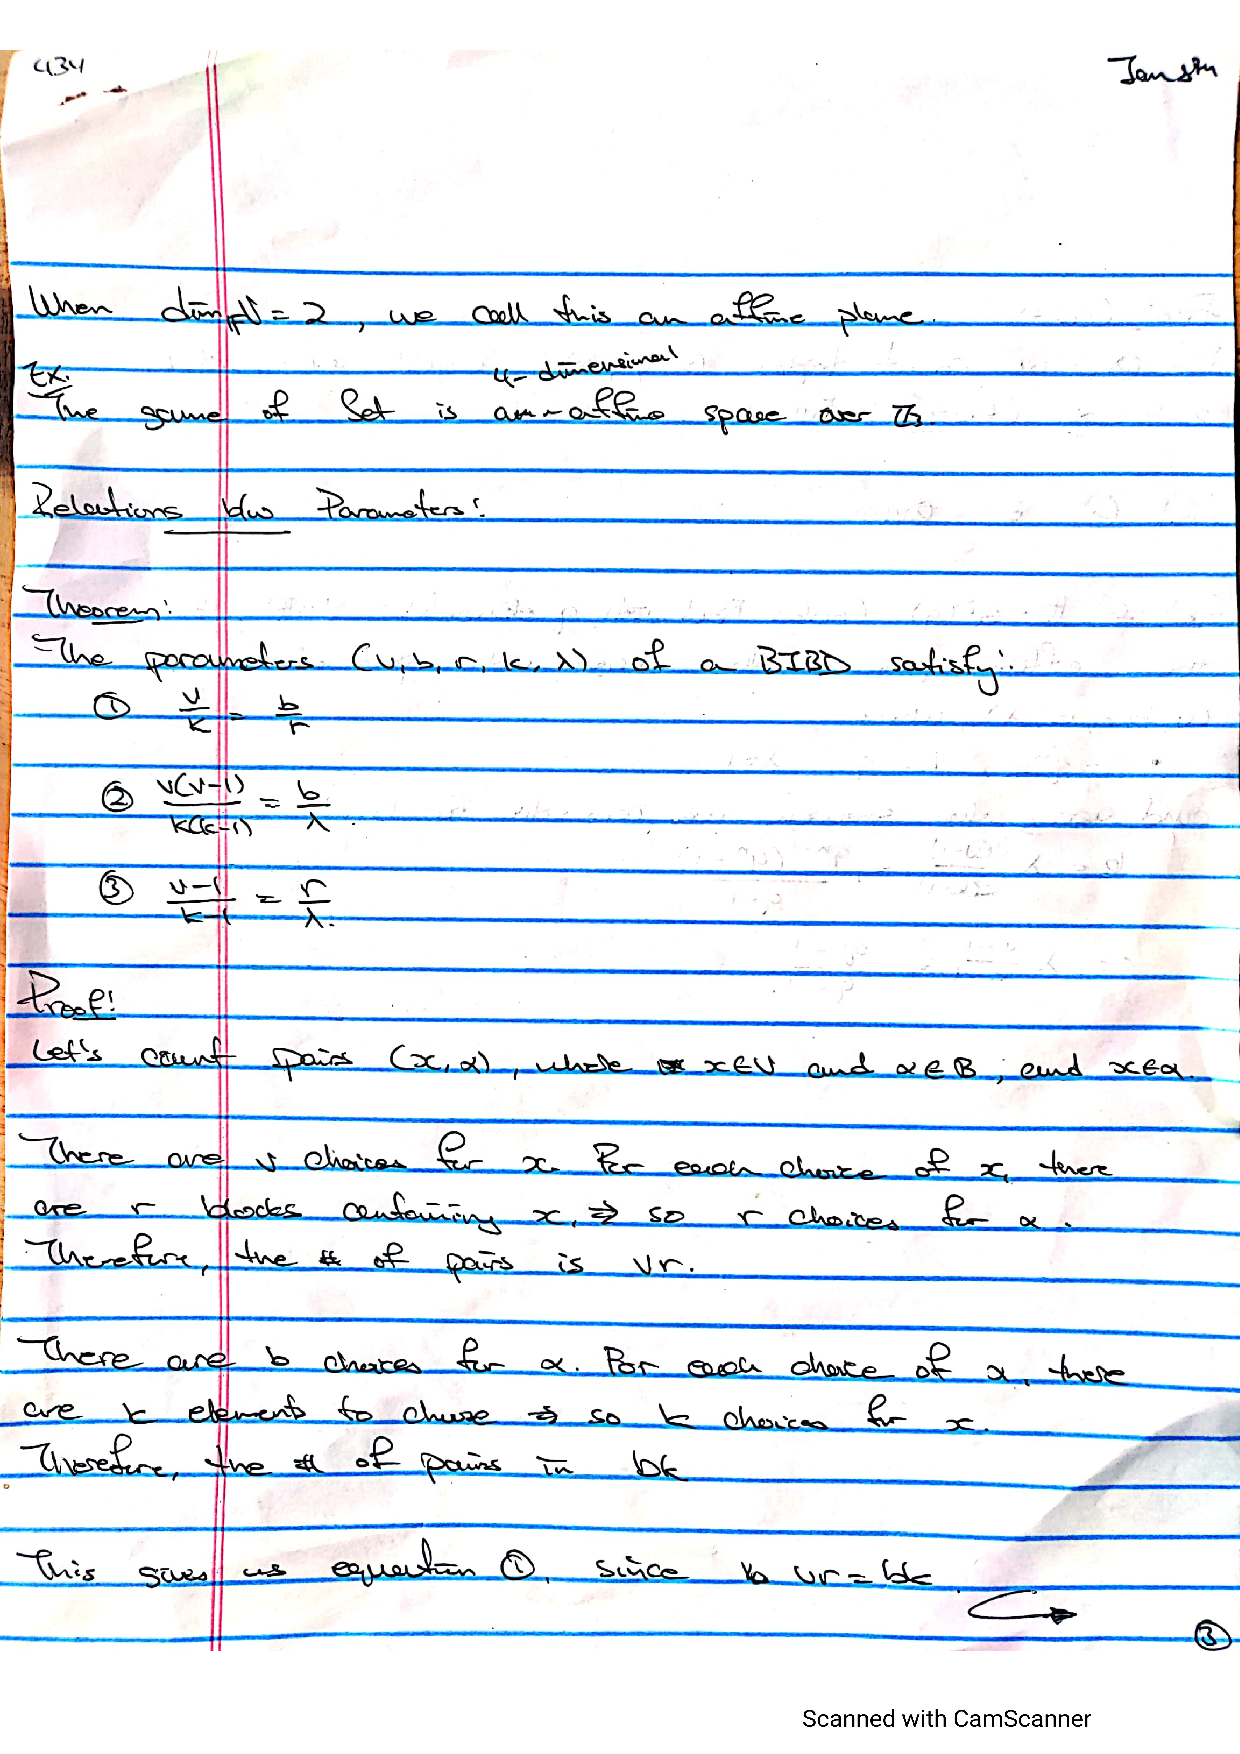
\includepdf[pages=-]{sections/lec2.pdf}\clearpage

Uploading scans of my notes for now ... I'll type these up one day ... 
\clearpage

\newcount\lecNum
\lecNum=3
\loop
  \includelecture{\the\lecNum}
  \advance \lecNum +1
\ifnum \lecNum<19
\repeat

\section*{}
Missed a definition in lecture 15 (there's a big blank chunk):

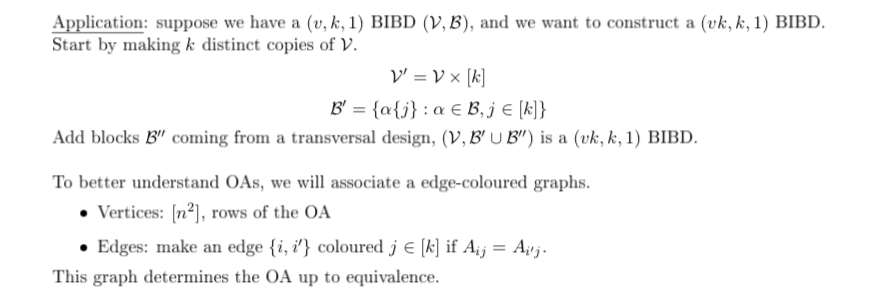
\includegraphics[width=\textwidth]{sections/lec15.png}
\clearpage

\nocite{*}
\bibliographystyle{unsrt}
\bibliography{co434}

\end{document}
